\begin{figure}[t]
\centering
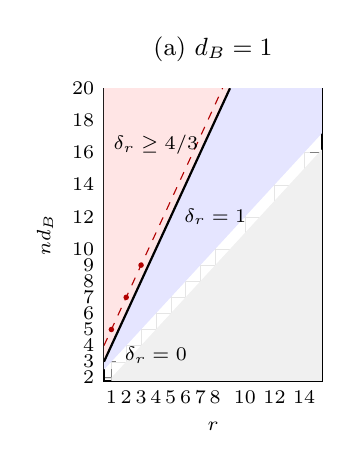
\begin{tikzpicture}
\begin{axis}[
    width=4.35cm, height=5.3cm,
    xlabel={$r$}, ylabel={$nd_B$},
    xmin=0.5, xmax=15.2, ymin=1.8, ymax=20,
    xtick={1,2,3,4,5,6,7,8,10,12,14},
    ytick={2,3,4,5,6,7,8,9,10,12,14,16,18,20},
    grid=both, grid style={line width=.1pt, draw=gray!20},
    tick label style={font=\scriptsize}, label style={font=\scriptsize},
    title={(a) $d_B=1$}, title style={font=\small}
]
\fill[gray!12] (axis cs:1,1.8) -- (axis cs:15.2,1.8) -- (axis cs:15.2,16.2) -- (axis cs:1,2) -- cycle;
\fill[blue!10] (axis cs:0.5,2.5) -- (axis cs:0.5,3) -- (axis cs:9,20) -- (axis cs:15.2,20) -- (axis cs:15.2,17.2) -- cycle;
\fill[red!10] (axis cs:0.5,3) -- (axis cs:0.5,20) -- (axis cs:9,20) -- cycle;
\draw[thick] (axis cs:0.5,3) -- (axis cs:9,20);
\draw[dashed, red!70!black] (axis cs:0.5,4) -- (axis cs:8.5,20);
\fill[red!70!black] (axis cs:1,5) circle (1.0pt);
\fill[red!70!black] (axis cs:2,7) circle (1.0pt);
\fill[red!70!black] (axis cs:3,9) circle (1.0pt);
\node[font=\scriptsize] at (axis cs:4,16.5) {$\delta_r\ge4/3$};
\node[font=\scriptsize] at (axis cs:8,12) {$\delta_r=1$};
\node[font=\scriptsize] at (axis cs:4,3.4) {$\delta_r=0$};
\end{axis}
\end{tikzpicture}
\hfil
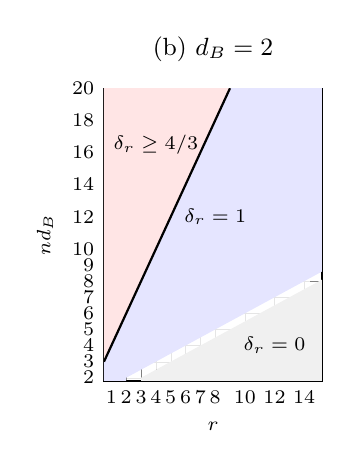
\begin{tikzpicture}
\begin{axis}[
    width=4.35cm, height=5.3cm,
    xlabel={$r$}, ylabel={$nd_B$},
    xmin=0.5, xmax=15.2, ymin=1.8, ymax=20,
    xtick={1,2,3,4,5,6,7,8,10,12,14},
    ytick={2,3,4,5,6,7,8,9,10,12,14,16,18,20},
    grid=both, grid style={line width=.1pt, draw=gray!20},
    tick label style={font=\scriptsize}, label style={font=\scriptsize},
    title={(b) $d_B=2$}, title style={font=\small}
]
\fill[gray!12] (axis cs:3,1.8) -- (axis cs:15.2,1.8) -- (axis cs:15.2,8.1) -- (axis cs:3,2) -- cycle;
\fill[blue!10] (axis cs:0.5,1.8) -- (axis cs:0.5,3) -- (axis cs:9,20) -- (axis cs:15.2,20) -- (axis cs:15.2,8.6) -- (axis cs:2,2) -- (axis cs:2,1.8) -- cycle;
\fill[red!10] (axis cs:0.5,3) -- (axis cs:0.5,20) -- (axis cs:9,20) -- cycle;
\draw[thick] (axis cs:0.5,3) -- (axis cs:9,20);
\node[font=\scriptsize] at (axis cs:4,16.5) {$\delta_r\ge4/3$};
\node[font=\scriptsize] at (axis cs:8,12) {$\delta_r=1$};
\node[font=\scriptsize] at (axis cs:12,4) {$\delta_r=0$};
\end{axis}
\end{tikzpicture}
\hfil
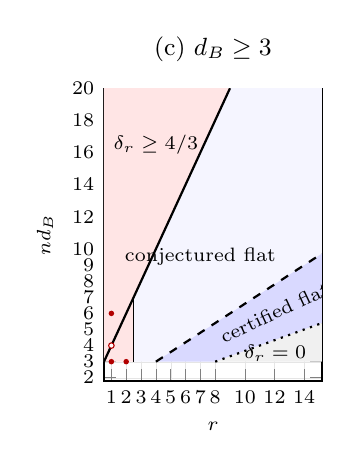
\begin{tikzpicture}
\begin{axis}[
    width=4.35cm, height=5.3cm,
    xlabel={$r$}, ylabel={$nd_B$},
    xmin=0.5, xmax=15.2, ymin=1.8, ymax=20,
    xtick={1,2,3,4,5,6,7,8,10,12,14},
    ytick={2,3,4,5,6,7,8,9,10,12,14,16,18,20},
    grid=both, grid style={line width=.1pt, draw=gray!20},
    tick label style={font=\scriptsize}, label style={font=\scriptsize},
    title={(c) $d_B\ge3$}, title style={font=\small}
]
\fill[red!10] (axis cs:0.5,3) -- (axis cs:0.5,20) -- (axis cs:9,20) -- cycle;
\fill[red!10] (axis cs:0.5,3) -- (axis cs:2.5,7) -- (axis cs:2.5,3) -- cycle;
\fill[blue!4] (axis cs:2.5,7) -- (axis cs:9,20) -- (axis cs:15.2,20) -- (axis cs:15.2,9.72) -- (axis cs:4,3) -- (axis cs:2.5,3) -- cycle;
\fill[blue!15] (axis cs:4,3) -- (axis cs:15.2,9.72) -- (axis cs:15.2,5.4) -- (axis cs:8,3) -- cycle;
\fill[gray!12] (axis cs:8,3) -- (axis cs:15.2,3) -- (axis cs:15.2,5.4) -- cycle;
\draw[thick] (axis cs:0.5,3) -- (axis cs:9,20);
\draw[dashed, thick] (axis cs:4,3) -- (axis cs:15.2,9.72);
\draw[dotted, thick] (axis cs:8,3) -- (axis cs:15.2,5.4);
\draw (axis cs:2.5,3) -- (axis cs:2.5,7);
\fill[red!70!black] (axis cs:1,3) circle (1.0pt);
\fill[red!70!black] (axis cs:2,3) circle (1.0pt);
\fill[red!70!black] (axis cs:1,6) circle (1.0pt);
\draw[red!70!black, fill=white] (axis cs:1,4) circle (1.0pt);
\node[font=\scriptsize] at (axis cs:4,16.5) {$\delta_r\ge4/3$};
\node[font=\scriptsize] at (axis cs:7,9.5) {conjectured flat};
\node[font=\scriptsize, rotate=25] at (axis cs:12,6.05) {certified flat};
\node[font=\scriptsize, anchor=east] at (axis cs:14.8,3.5) {$\delta_r=0$};
\end{axis}
\end{tikzpicture}
\caption{Flat-width regimes of the input-independent body ($d_A=1$, $nd_B>2$) in the plane of the latent dimension $r$ and the flag-coordinate count $nd_B$; the solid line in every panel is the phase boundary $nd_B=2r+2$. The drawings are schematic: the regions are exact at the lattice points of each panel within the subcritical range $1\le r\le nd_B^2-2$ where the classification statements apply (from the affine dimension on, the width is zero, Theorem~\ref{thm:zero-error}); in (a) $nd_B=n$, in (b) $nd_B=2n$, and in (c) $nd_B\ge3$ with the dashed and dotted boundaries drawn for $d_B=3$. (a) Classical outputs: $\delta_r=1$ between the boundary and the exact-reconstruction region, $\delta_r\ge4/3$ above the boundary (Corollaries~\ref{cor:classical-dichotomy} and~\ref{cor:flat-fails}); on the dashed line $nd_B=2r+3$ the value is exactly $4/3$ (Corollary~\ref{cor:exact-d1}), marked at $(r,nd_B)=(1,5),(2,7),(3,9)$; the row $nd_B=2$ is the collapse case (i) of Theorem~\ref{thm:collapse}. (b) Qubit outputs: $\delta_r=1$ for $r\ge n-1$, equivalently below the boundary, and $\delta_r\ge4/3$ above it (Corollary~\ref{cor:qubit-dichotomy}); the row $nd_B=2$ is the collapse case (ii) of Theorem~\ref{thm:collapse}. (c) Outputs with $d_B\ge3$: $\delta_r\ge4/3$ above the boundary (Corollary~\ref{cor:flat-fails}) and in the columns $r\in\{1,2\}$, where the state-space obstruction applies at every $n$ (Theorems~\ref{thm:state-nonflat} and~\ref{thm:state-d2} with the concentration gate of Lemma~\ref{lem:slice-gate}); below the boundary at $r\ge3$, flatness is conjectured (Conjecture~\ref{con:coord-flat}), certified beyond the dashed pinching boundary $r=nQ_2(d_B)-1$ (Theorem~\ref{thm:pinching}; $Q_2(3)=5$ by the balanced two-sector split), the strip between the two boundaries being open (Remark~\ref{rem:flat-status}). Filled circles mark instances with value exactly $4/3$: $(1,5)$ in (a) ($n=5$), and in (c) the qutrit at $(1,3)$ and $(2,3)$ ($n=1$) together with $(1,6)$ ($n=2$, where $2(1-1/3)=4/3$, Theorem~\ref{thm:mass-exact}); the open circle marks the one-outcome ququart at $(1,4)$, where $\delta_1\in[4/3,3/2]$ (Corollary~\ref{cor:bottom-dichotomy}).}
\label{fig:flat-regimes}
\end{figure}
